% Chapter 4

\chapter{Case Study} % Main chapter title

\label{Chapter4} % For referencing the chapter elsewhere, use \ref{Chapter1} 

\lhead{4. \emph{Case Study}} % This is for the header on each page - perhaps a shortened title

\begin{figure}[!htpb]
	\centering
		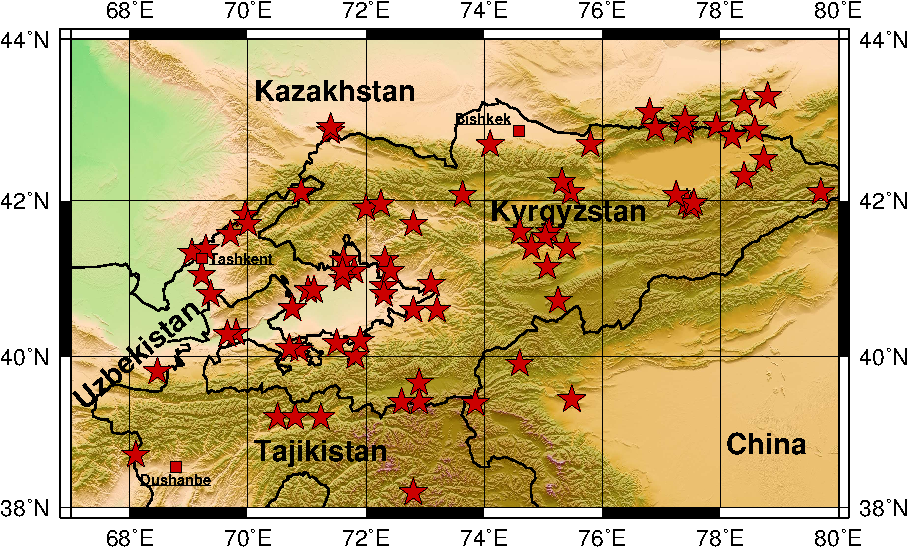
\includegraphics[scale=0.9]{Figures/CentralAsia.pdf}
		\rule{35em}{0.5pt}
	\caption[map]{map}
	\label{fig:map}
\end{figure}

\section{Data}


\begin{table}[ht]
  \centering
        \small
        \setlength\tabcolsep{2pt}
\begin{tabular}{|r|r|r|r|r|r|r|r|r|r|r|r|r|r|r|r|r||r|}
  \hline
$I_0 / I_s$ & 1.5 & 2 & 2.5 & 3 & 3.5 & 4 & 4.5 & 5 & 5.5 & 6 & 6.5 & 7 & 7.5 & 8 & 8.5 & 9 & total \\ 
  \hline
9 & 0 & 0 & 0 & 0 & 13 & 4 & 25 & 23 & 34 & 15 & 23 & 13 & 17 & 4 & 13 & 3 & 187 \\ 
  8.5 & 0 & 0 & 11 & 10 & 62 & 13 & 142 & 33 & 147 & 25 & 153 & 90 & 98 & 14 & 110 & 0 & 908 \\ 
  8 & 0 & 0 & 24 & 9 & 24 & 8 & 48 & 18 & 47 & 28 & 26 & 10 & 9 & 5 & 0 & 0 & 256 \\ 
  7.5 & 3 & 16 & 33 & 68 & 198 & 186 & 204 & 133 & 116 & 76 & 91 & 23 & 24 & 0 & 0 & 0 & 1171 \\ 
  7 & 4 & 24 & 69 & 75 & 149 & 132 & 139 & 67 & 79 & 29 & 29 & 9 & 0 & 0 & 0 & 0 & 805 \\ 
  6.5 & 1 & 15 & 104 & 98 & 219 & 146 & 129 & 60 & 118 & 71 & 56 & 0 & 0 & 0 & 0 & 0 & 1017 \\ 
  6 & 17 & 26 & 103 & 131 & 189 & 86 & 105 & 64 & 90 & 34 & 0 & 0 & 0 & 0 & 0 & 0 & 845 \\ 
  5.5 & 0 & 22 & 155 & 116 & 233 & 166 & 147 & 46 & 70 & 0 & 0 & 0 & 0 & 0 & 0 & 0 & 955 \\ 
  5 & 8 & 1 & 9 & 23 & 19 & 7 & 5 & 5 & 0 & 0 & 0 & 0 & 0 & 0 & 0 & 0 & 77 \\ 
  \hline
  total & 33 & 104 & 508 & 530 & 1106 & 748 & 944 & 449 & 701 & 278 & 378 & 145 & 148 & 23 & 123 & 3 & 6221 \\ 
   \hline
\end{tabular}
\caption[Data]{Data}
\label{table:Data}
\end{table}

\section{Handling uncertain data}

sdavasgas
\begin{table}[ht]
\centering
\begin{tabular}{rrrrrrr}
  \hline
 $I_0$& round & floor & ceiling & Certain & Inflated & Inflated Uncertain \\ 
  \hline 
  5 & - & \cellcolor{green!25}0.493506 & - & - & 0.571429 & \cellcolor{red!25}0.584416 \\ 
  6 & 0.553543 & 0.541667 & \cellcolor{green!25}0.496124 & 0.489256 & 0.566914 & \cellcolor{red!25}0.584479 \\ 
  7 & 0.660767 & \cellcolor{green!25}0.656970 & 0.677229 & 0.681021 & \cellcolor{red!25}0.695033 & 0.679183 \\ 
  8 & 0.556452 & \cellcolor{green!25}0.504555 & \cellcolor{red!25}0.601721 & 0.521674 & 0.593300 & 0.544509 \\ 
  9 & 0.748899 & 0.743379 & \cellcolor{red!25}0.816151 & \cellcolor{green!25}0.697095 & 0.807437 & 0.787307 \\ 
  10 & \cellcolor{red!25}0.620321 & - & \cellcolor{green!25}0.582888 &-  & 0.604278 & 0.614973 \\ 
   \hline
\end{tabular}
\caption[Data]{Data}
     \label{table:Rotondi}
\end{table}

\section{Comparison to other studies}


\begin{table}[!ht]
\centering
\begin{tabular}{rrr}
  \hline
 $I_0$& Rotondi & Ullah \\ 
  \hline
  5 & \cellcolor{green!25}0.493506  & \cellcolor{red!25}0.934634\\ 
  6 & \cellcolor{green!25} 0.541667 & \cellcolor{red!25}0.613935 \\ 
  7 & \cellcolor{green!25}0.656970  & \cellcolor{red!25}0.570863 \\ 
  8 & \cellcolor{green!25}0.504555 & \cellcolor{red!25}0.562258  \\ 
  9 & \cellcolor{red!25}0.743379 & \cellcolor{green!25}0.743313  \\ 
  10 & - & - \\ 
   \hline
   \end{tabular}
\caption[Data]{Data}
     \label{table:Ullah}
\end{table}

\section{Extended Source}